\documentclass[dvipdfmx,8pt]{beamer}


\usepackage{here, amsmath, latexsym, amssymb, bm, ascmac, mathtools, multicol, tcolorbox, subfig,color}
\usepackage{tikz}
\usepackage{graphicx}
\renewcommand{\baselinestretch}{1.5}
\renewcommand{\figurename}{図}
\renewcommand{\tablename}{表}
\renewcommand\mathfamilydefault{\rmdefault}
\setbeamertemplate{navigation symbols}{}

\usetheme{Boadilla}

\title{ディープラーニング基礎}
\subtitle{Chapter2 \ 機械学習と深層学習}
\author[須賀]{須賀勇貴}
\institute[茨大]{茨城大学大学院 \ 理工学研究科 \ 量子線科学専攻 \ 1年}
\date{\today}

\begin{document}

\frame{\maketitle}

  \begin{frame}{2.1 \ なぜ深層学習か?}
    \begin{figure}
      \begin{center}
        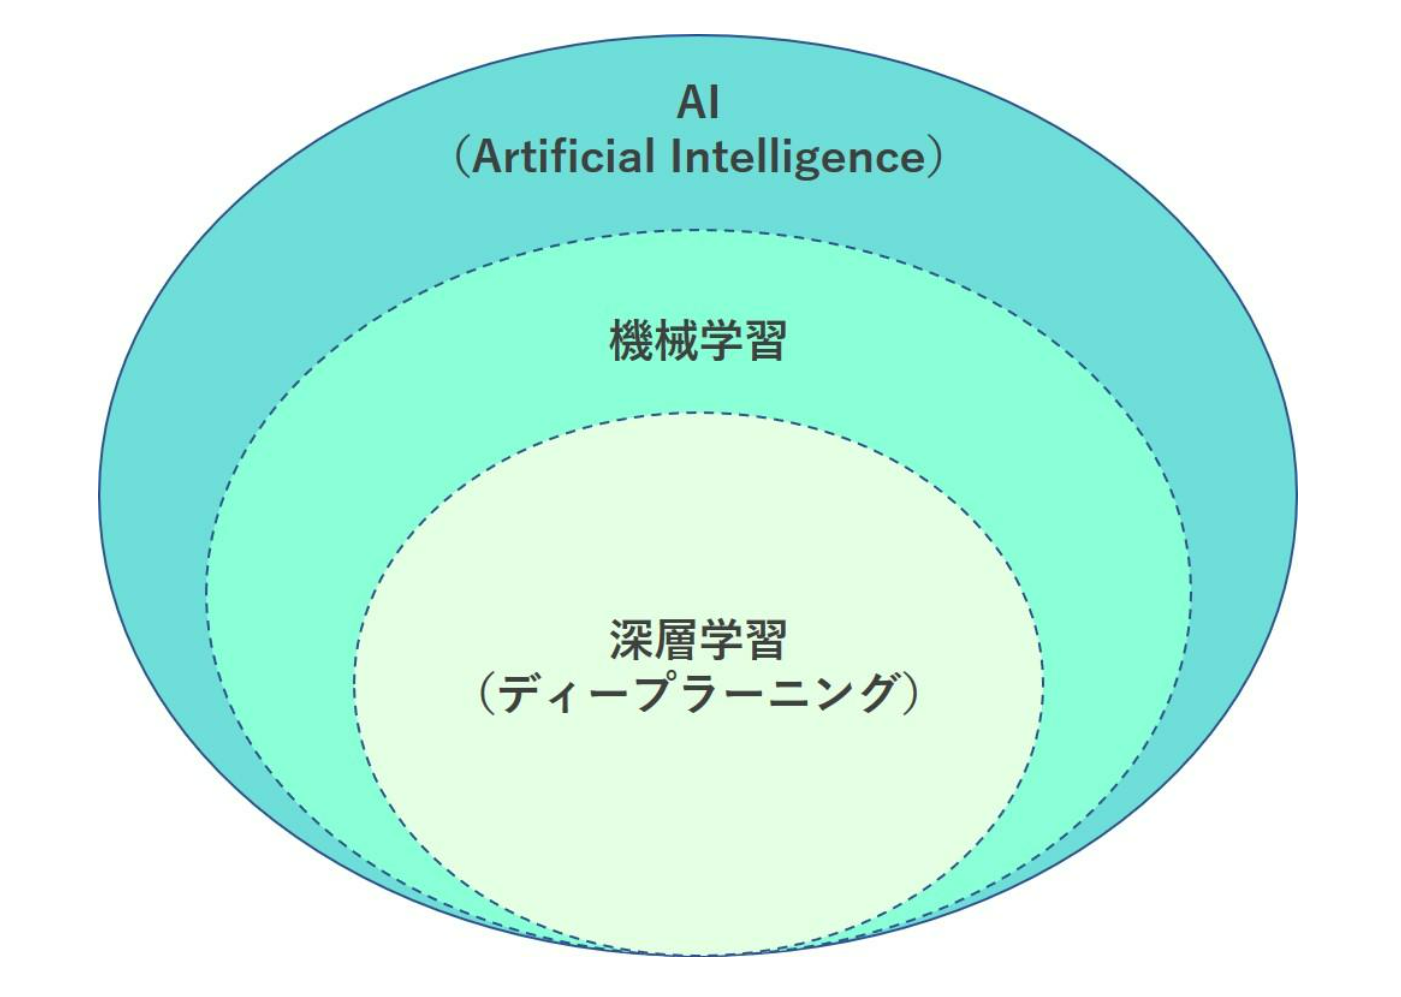
\includegraphics[height=6cm]{./AI_ML_DL.png}
      \end{center} 
      \caption{AIと機械学習とディープラーニングの関係}  
    \end{figure}
    https://business.ntt-east.co.jp/content/cloudsolution/column-159.html
  \end{frame}

  \begin{frame}{2.1 \ なぜ深層学習か?}
    \begin{block}{深層学習(Deep Learning)とは}
      動物の神経回路にヒントを得て提唱された\textbf{(深層)ニューラルネットワーク}計算により,\\
      大量のデータからその背後に潜む知識を自発的に獲得していく手法
    \end{block}
    \begin{columns}
      \begin{column}{0.5\textwidth}
        \begin{itemize}
          \item 深層学習の何がすごい?
          \vspace{0.3cm}
          \begin{enumerate}
            \item 汎用的なアルゴリズムを提案してくれる\\
            $\rightarrow$ タスクの種類に依存しない
            \vspace{0.3cm}
            \item 極めて高い汎化性能がある\\
            $\rightarrow$ 手持ちのデータだけの中から,全ての状況に通用する本質的な知識を獲得できる
          \end{enumerate}
        \end{itemize}
      \end{column}
      \begin{column}{0.5\textwidth}
        \begin{figure}
          \begin{center}
            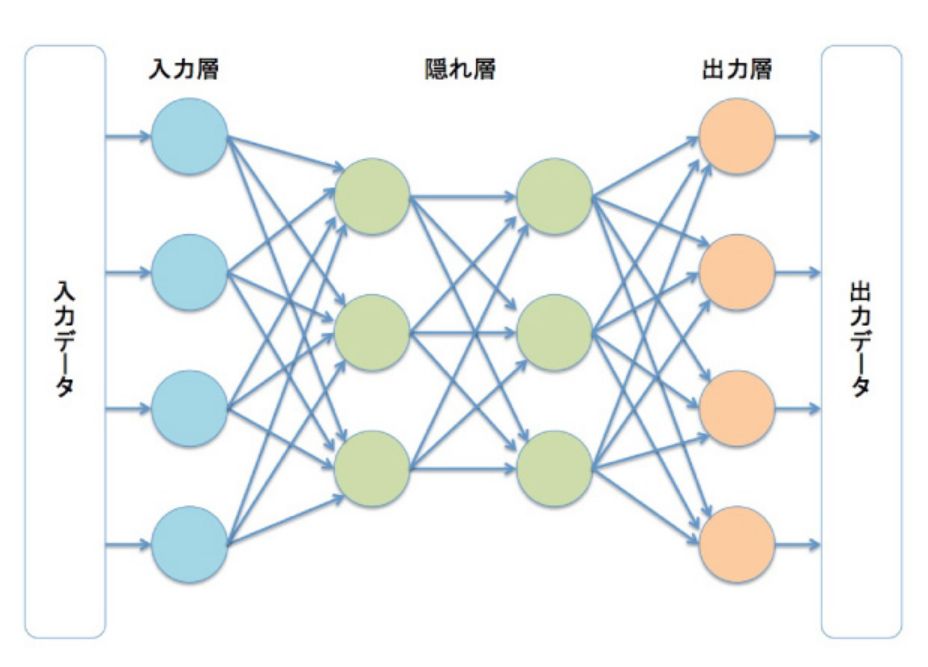
\includegraphics[height=4cm]{./NN.png}
          \end{center} 
          \caption{深層ニューラルネットラークの図}  
        \end{figure}
      \end{column}
    \end{columns}
    
  \end{frame}

  \begin{frame}{2.2 \ 機械学習とは何か}
    機械学習とは,人間がこなすようなさまざまな学習や知的作業を計算機に実行させるためのアプローチの研究,あるいはその手法そのものを意味する
    \begin{block}{T. M. ミッシェルによる機械学習の定式化}
      「コンピュータプログラムが,ある種の\textbf{タスクT}と\textbf{評価尺度P}において\textbf{経験E}から学習するとは,\textbf{タスクT}におけるその性能を\textbf{評価尺度P}によって評価した際に,\textbf{経験E}によってそれが改善されている場合である」
    \end{block}
    タスクT $\cdots$ 解きたい問題.\\
    \hspace{1.7cm}例)回帰,分類,強化学習,パターン認識,クラスタリング分析,最適化分析など\\
    評価尺度P $\cdots$ モデルの精度.\\
    \hspace{2cm}回帰の場合,「平均二乗誤差」がよく使われる\\
    経験E $\cdots$ データ集合.\\
    \begin{itembox}[l]{要するに}
    経験Eの蓄積によってタスクTを解いたときに,評価尺度Pが向上する手法
    \end{itembox}
  \end{frame}

  \begin{frame}{2.2 \ 機械学習とは何か \\ \normalsize{2.2.1 \ 代表的なタスク}}
    \begin{block}{(1)クラス分類}
      いくつかのカテゴリ(クラス)に仕分ける作業\\
      与えられた数値データを$\bm{x}$,クラス($K$個)を$\mathcal{C}_y \ (y = 0,1,\cdots,K)$で表すことにすると,$\bm{x}$をクラス$\mathcal{C}_y$へ分離するということは,$\bm{x}$の所属クラスを表す離散値ラベル$\bm{y}$の値を決めることである
      \begin{equation*}
        \bm{x} \rightarrow \bm{y}(\bm{x}) \in \{0 , 1 , \cdots , K\}
      \end{equation*}
    \end{block}
    \begin{block}{(2)回帰}
      データから,それに対応する実数値(を並べたベクトル)$\bm{y}$を予測する作業.つまり,与えられた$\bm{x}$を,対応する$\bm{y}$に変換するための関数$\bm{y}(\bm{x})$を決定する
      \begin{equation*}
        \bm{x} \rightarrow \bm{y}(\bm{x}) \in \mathbb{R}
      \end{equation*} 
    \end{block}
       
    \begin{exampleblock}{回帰におけるタスクの応用例}
      機械翻訳,音声認識,異常検知,データ次元削除
    \end{exampleblock}
  \end{frame}

  \begin{frame}[t]{2.2 \ 機械学習とは何か \\ \normalsize{2.2.2 \ さまざまなデータセット}}
    \begin{columns}
      \begin{column}{0.5\textwidth}
        MNIST
        \begin{figure}
          \begin{center}
            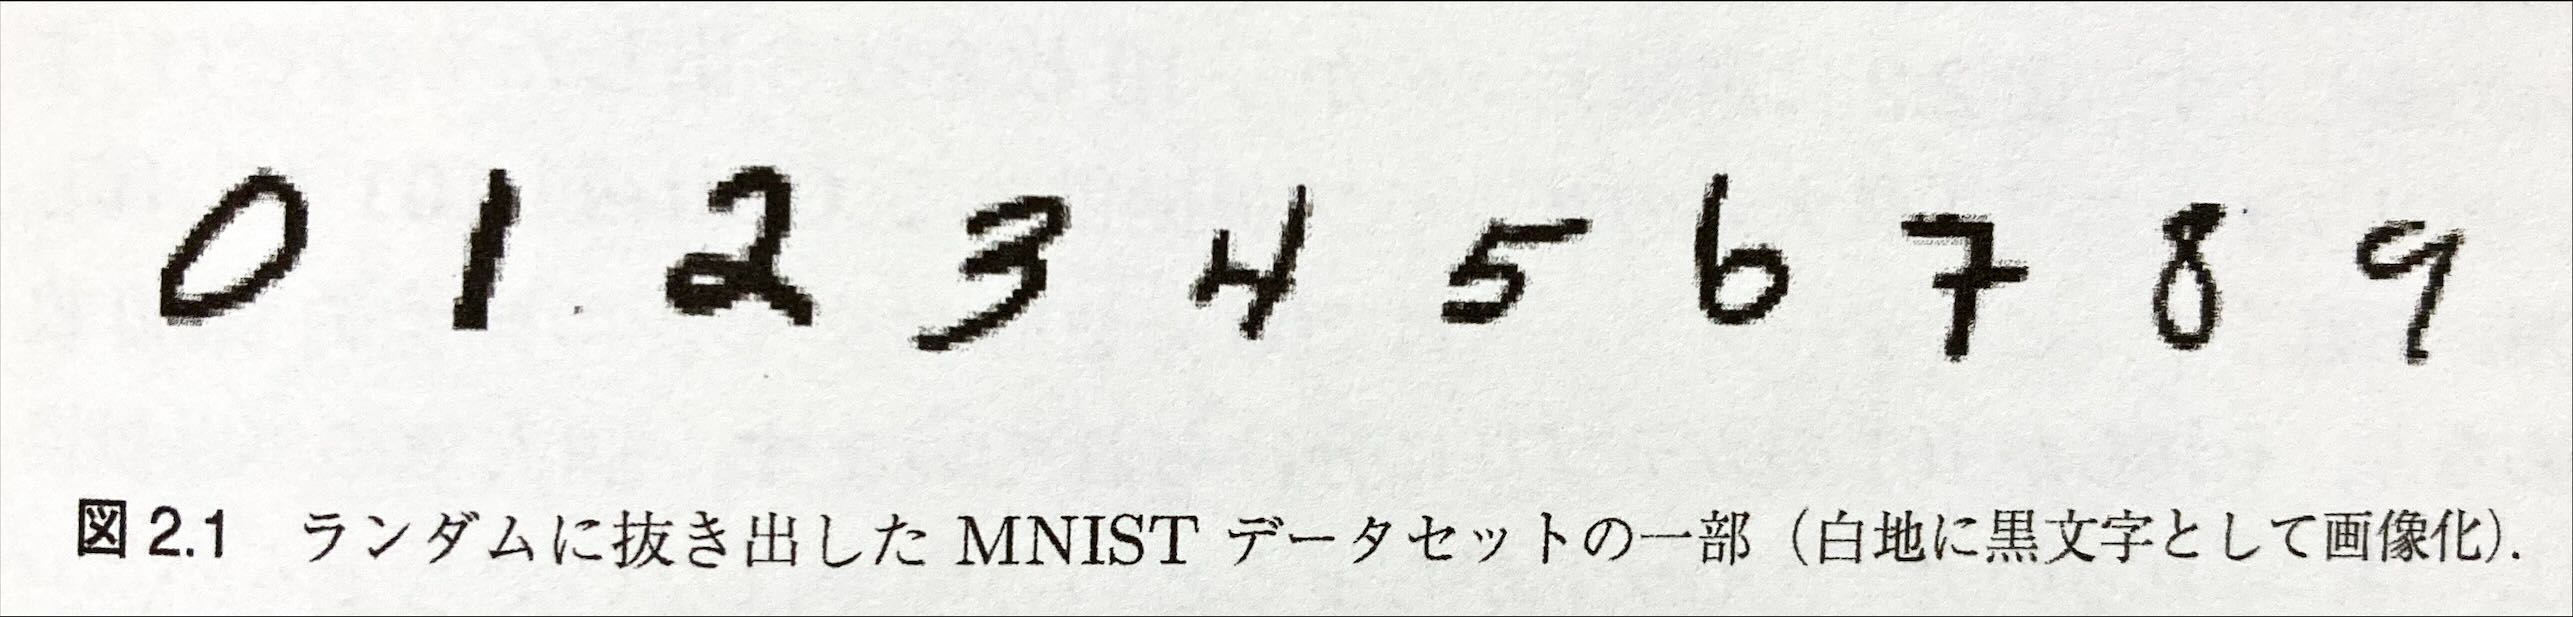
\includegraphics[height=1.2cm]{./MNIST.jpeg}
          \end{center}   
        \end{figure}
        \begin{itemize}
          \item 手書き数字のデータベース
          \item グレースケールの$28 \times 28$ピクセル画像
          \item 訓練用に6万枚,テスト用に1万枚用意されている
        \end{itemize}
        Imagenet
        \begin{itemize}
          \item 約1400万枚の自然画像からなる巨大データベース
          \item クラス数は2万にも及ぶ
        \end{itemize}
      \end{column}
      \begin{column}{0.5\textwidth}
        CIFAR-10
        \begin{figure}
          \begin{center}
            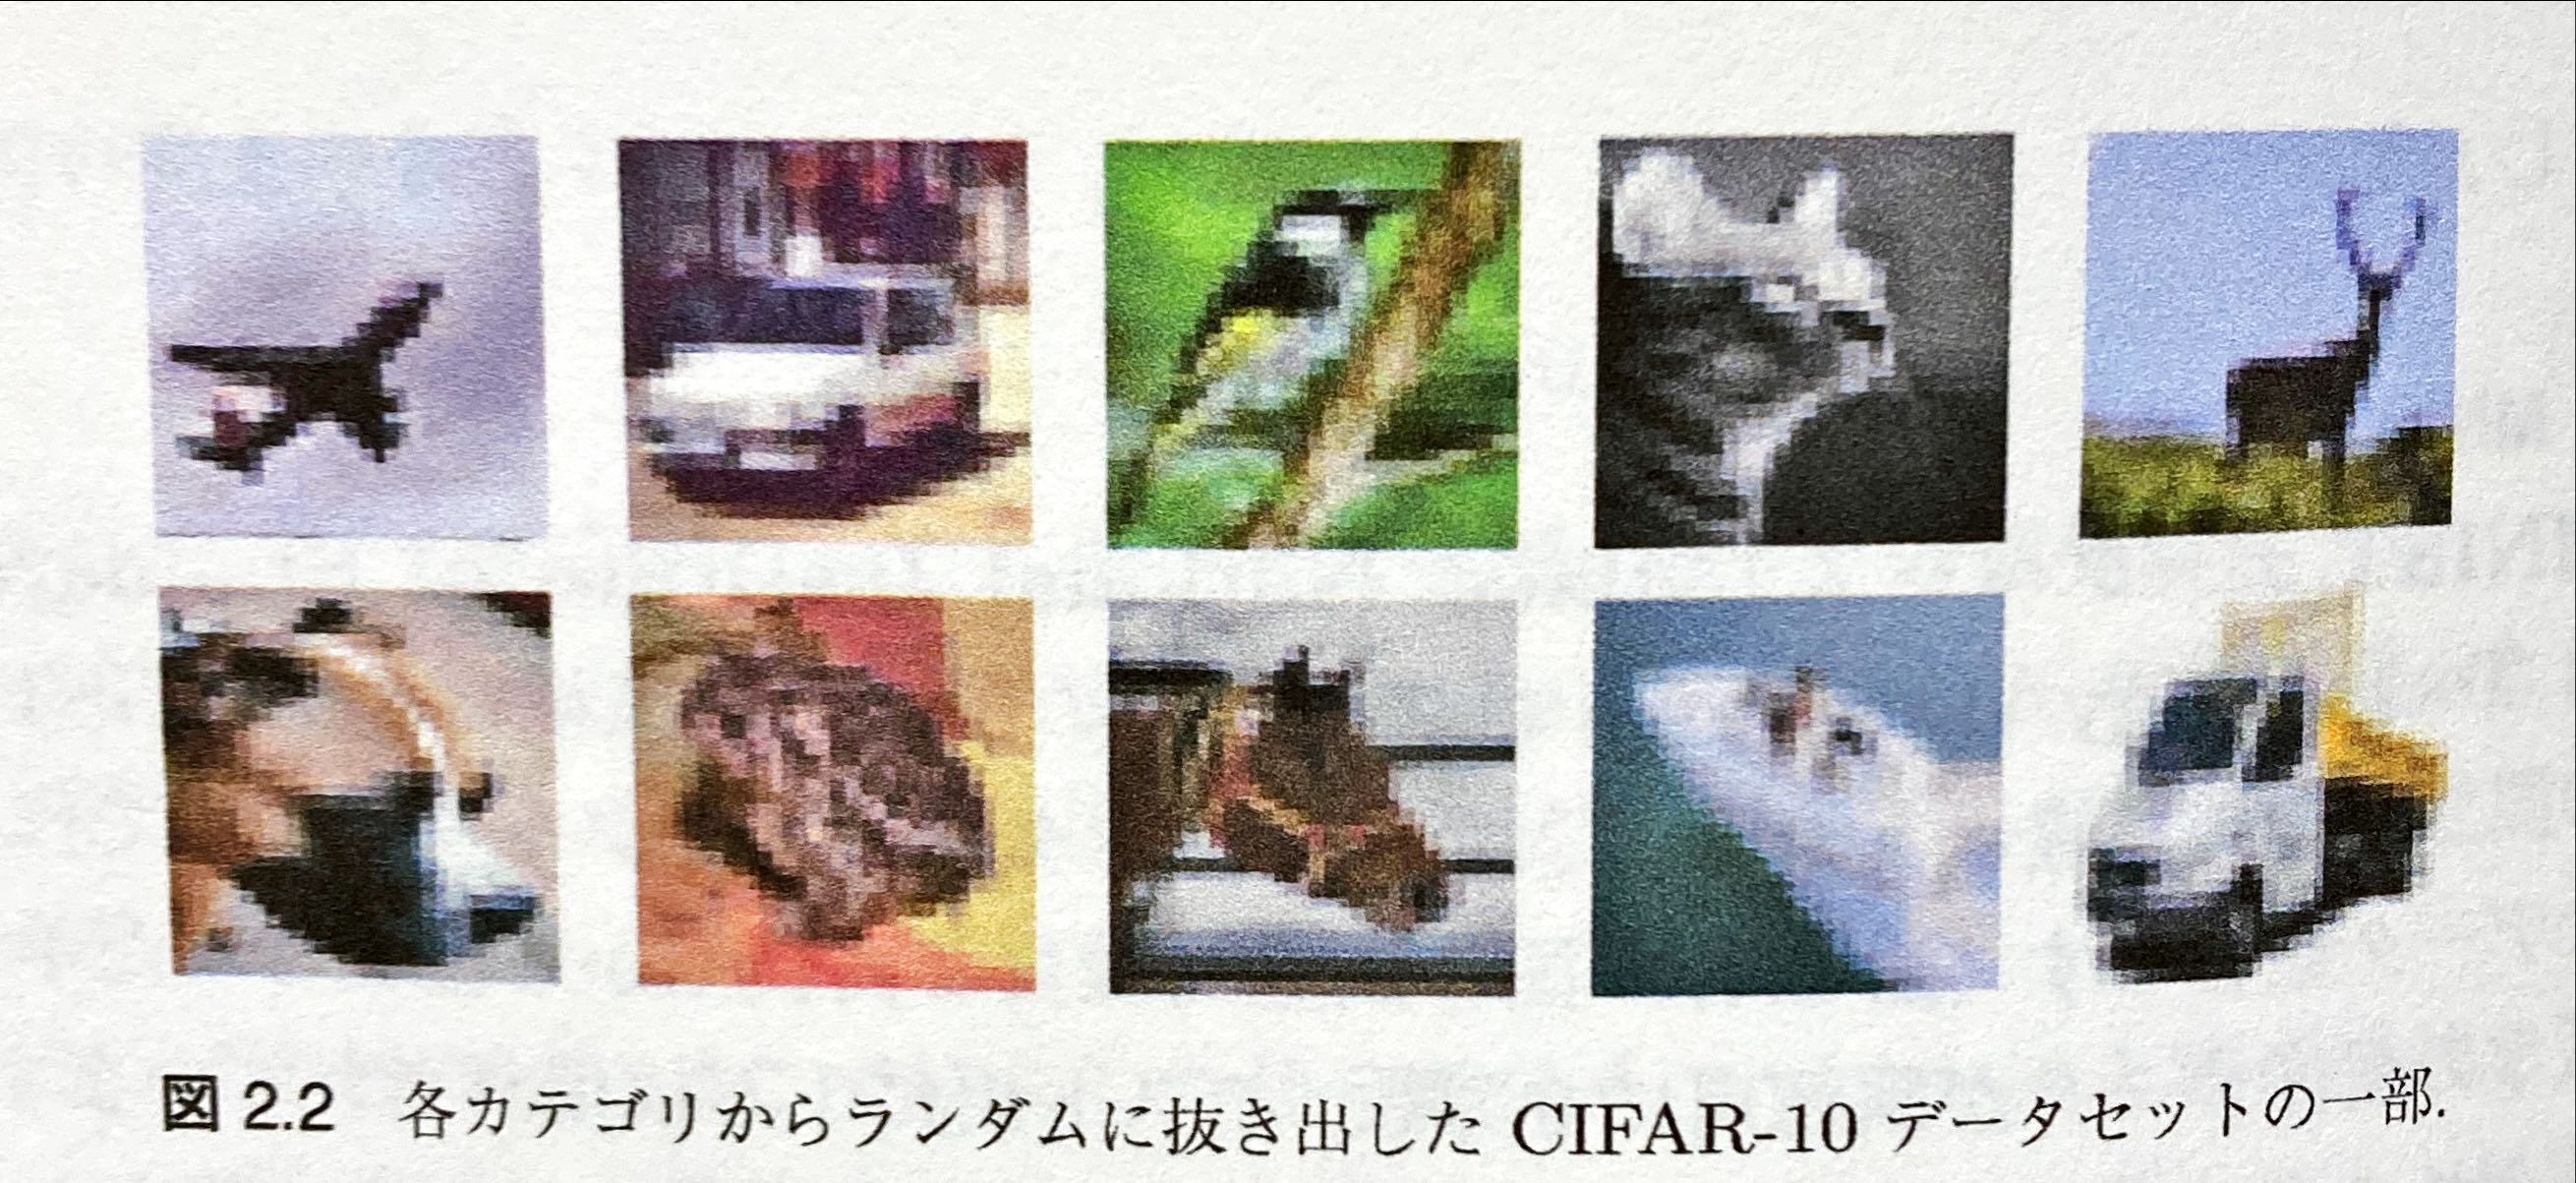
\includegraphics[height=2.5cm]{./CIFAR10.jpeg}
          \end{center}   
        \end{figure}
        \begin{itemize}
          \item 自然画像のデータベース
          \item 10のカテゴリに分けられた$32 \times 32$ピクセル画像
          \item 訓練用に6万枚,テスト用に1万枚用意されている
        \end{itemize}
      \end{column}
    \end{columns}
  \end{frame}


  \begin{frame}{2.3 \ 統計入門 \\ \normalsize{2.3.1 \ 標本と推定}}
    どのようにしたらプログラムはデータからタスクをこなすための知識を学び取れるか?\\
    \begin{center}
      データを科学的に分析 $\rightarrow$ 統計学
    \end{center}
    機械学習の手法も統計を基礎として構築される(統計的機械学習)\\
    まずは用語の確認\\
    \begin{center}
      \textbf{データ(集合)}や\textbf{サンプル,標本} $\cdots$ \textbf{データ点(data point)}の集まりからなるもの\\
    \end{center}
    \begin{exampleblock}{手書き文字画像認識の例}
      \begin{center}
        データ(集合) $\rightarrow$ 画像の集合\\
        データ点 $\rightarrow$ 1枚1枚の画像
      \end{center}
    \end{exampleblock}
    \vspace{0.2cm}
    ※これらの用語は乱用されており,データ点を略してデータと言ったり,サンプルをサンプルの要素であるデータ点の意味で用いたりする\\
    \begin{center}
      $\rightarrow$ 文脈から意味を判断
    \end{center}
  \end{frame}

  \begin{frame}[t]{2.3 \ 統計入門 \\ \normalsize{2.3.1 \ 標本と推定}}
    \textbf{推定}を考える\\
    \begin{itemize}
      \item 統計解析に用いるデータは母集団から無作為に抽出されたものとみなす
      \item データの分析から母集団についての知識を獲得することが目標
      \item 母集団の性質はデータ生成確率$P_{data}(\bm{x})$により特徴付けられているものとする(=不確定性のある現象を確率的にモデル化)
      \item サンプル$\bm{x}$はデータ生成確率から抽出されたものであると仮定する
    \end{itemize}
    \begin{equation*}
      \bm{x} \sim P_{data}(\bm{\mathrm{x}})
    \end{equation*}
    $\rightarrow$ 現象を確率的に予測できるようになる
  \end{frame}

  \begin{frame}[t]{2.3 \ 統計入門 \\ \normalsize{2.3.1 \ 標本と推定}}
    \textbf{推定}を考える\\
    \begin{center}
      母集団について知る = データ生成分布を知る
    \end{center}
    データ生成分布を特徴づける量を\textbf{パラメータ}と呼ぶ
    \begin{exampleblock}{ガウス分布の例}
      パラメータは平均値$\mu$と分散$\sigma^2$
      \begin{equation*}
        P(x)=\mathcal{N}(x;\mu,\sigma^2)=\frac{1}{\sqrt{2\pi \sigma^2}}e^{-\frac{(x-\mu)^2}{2\sigma^2}}
      \end{equation*}
      この2つの値が決まれば分布が具体的に決定される
    \end{exampleblock}
    実際のデータ生成分布は無数のパラメータを持つ
    $\rightarrow$ 良く近似できると期待できるモデル分布$P(\mathrm{X};\bm{\theta})$を仮定し,そのモデルのパラメータ$\bm{\theta}$の最適値$\bm{\theta}^*$をデータから推定する\\
    $\rightarrow$ パラメトリックなアプローチ
  \end{frame}

  \begin{frame}[t]{2.3 \ 統計入門 \\ \normalsize{2.3.2 \ 点推定}}
    \begin{block}{点推定とは}
      手持ちの有限要素のデータ集合$\mathcal{D}=\{x_1,x_2,\cdots,x_N\}$から確率分布のパラメータの尤もらしい値を計算すること
    \end{block}
    点推定のためには,データを決める確率変数$\{\mathrm{x_1},\mathrm{x_2},\cdots,\mathrm{x_N}\}$の関数である推定量を作る必要がある
    \begin{equation*}
      \hat{\bm{\theta}}(\mathrm{x_1},\mathrm{x_2},\cdots,\mathrm{x_N})
    \end{equation*}
    これに具体的なデータが与えられると,数値としてのパラメータの推定値を得られる
    \begin{equation*}
      \hat{\bm{\theta}}^*(x_1,x_2,\cdots,x_N) = \hat{\bm{\theta}}(x_1,x_2,\cdots,x_N)
    \end{equation*}
    この推定値は考えているパラメータを良く近似するように作る必要がある
  \end{frame}

  \begin{frame}[t]{2.3 \ 統計入門 \\ \normalsize{2.3.2 \ 点推定}}
    良い推定量の作り方
    \pause
    \begin{enumerate}
      \item バイアスが小さい \ \ バイアス$\cdots$推定量の期待値$E[\hat{\bm{\theta}}]$と真の値$\theta^*$の差
        \begin{equation*}
          b(\hat{\bm{\theta}}) = E[\hat{\bm{\theta}}] - \theta^*
        \end{equation*}
        \textbf{不偏推定量} $\cdots$ バイアスがゼロのもの(望ましい推定量)\\
        \textbf{漸近不偏推定量} $\cdots$ データの数が増えるにつれゼロへ漸近するもの($\lim_{N \rightarrow \infty}b(\hat{\bm{\theta}})=0$)
        \pause
      \item 分散が小さい(つまり,真の値に対して推定値のばらつきが小さい)
        \begin{equation*}
          Var(\hat{\bm{\theta}}) = E\left[\left(\hat{\bm{\theta}}-\bm{\theta}^*\right)^2\right]
        \end{equation*}
        \pause
      \item 一致性がある\\
        データ点の数が増えるにつれて統計量が真のパラメータに近づいていくという性質\\
        \textbf{一致推定量} $\cdots$ $N \rightarrow \infty$に従い$\hat{\bm{\theta}} \rightarrow \bm{\theta}^*$となる推定量
    \end{enumerate}
  \end{frame}

  \begin{frame}[t]{2.3 \ 統計入門 \\ \normalsize{2.3.2 \ 点推定}}
    (1) ガウス分布
    \begin{equation*}
      P(x)=\mathcal{N}(x;\mu,\sigma^2)=\frac{1}{\sqrt{2\pi \sigma^2}}e^{-\frac{(x-\mu)^2}{2\sigma^2}}
    \end{equation*}
    ガウス分布から無作為に取り出した$N$個のデータからパラメータを推定するにはどうしたらよいか?
    任意のデータ点$\mathrm{x}_n$の期待値
    \begin{equation*}
      E_{\mathcal{N}}[\mathrm{x}_n] = \int_{-\infty}^{\infty}x_n P(x_n) dx_n = \mu
    \end{equation*}
    $\rightarrow$ $\mu$の推定値$\hat{\mu}$をサンプル平均としてみる
    \begin{equation*}
      \hat{\mu} = \frac{1}{N}\sum_{n=1}^{N}\mathrm{x}_n
    \end{equation*}
    これは見事に不偏推定量となっている
    \begin{equation*}
      E_{\mathcal{N}}[\hat{\mu}] = \frac{1}{N}\sum_{n=1}^{N}E_{\mathcal{N}}[\mathrm{x}_n] =\mu
    \end{equation*}
  \end{frame}

  \begin{frame}[t]{2.3 \ 統計入門 \\ \normalsize{2.3.2 \ 点推定}}
    (1) ガウス分布
    \begin{equation*}
      P(x)=\mathcal{N}(x;\mu,\sigma^2)=\frac{1}{\sqrt{2\pi \sigma^2}}e^{-\frac{(x-\mu)^2}{2\sigma^2}}
    \end{equation*}
    ガウス分布から無作為に取り出した$N$個のデータからパラメータを推定するにはどうしたらよいか?
    $(\mathrm{x}_n - \mu)^2$の期待値
    \begin{equation*}
      E_{\mathcal{N}}[(\mathrm{x}_n - \mu)^2] = \int_{-\infty}^{\infty}(x_n - \mu)^2 P(x_n) dx_n = \sigma^2
    \end{equation*}
    $\rightarrow$ 平均値のときと同様に$\sigma^2$の推定値$\hat{\sigma}^2$をサンプル平均による近似で表す
    \begin{equation*}
      \hat{\sigma}^2 = \frac{1}{N}\sum_{n=1}^{N}(\mathrm{x}_n - \mu)^2
    \end{equation*}
    これは不偏推定量ではなく,漸近的不偏推定量になる
    \begin{equation*}
      E_{\mathcal{N}}[\hat{\sigma}^2] = \left( \frac{N}{N-1}\right)\sigma^2
    \end{equation*}
  \end{frame}

  \begin{frame}[t]{2.3 \ 統計入門 \\ \normalsize{2.3.2 \ 点推定}}
    (2) ベルヌーイ分布
    \begin{equation*}
      P(x)=p^x(1-p)^{1-x}
    \end{equation*}
    パラメータは$p$のみ.期待値と分散は以下
    \begin{align*}
      &E_P[\mathrm{x}] = \sum_{x=0,1}xP(x) = P(1) = p\\
      &E_P[(\mathrm{x}-p)^2] = \sum_{x=0,1}(x -2px +p^2)P(x) = p(1-p)
    \end{align*}
    $\rightarrow$ 推定量はサンプル平均とするのが良さそう
    \begin{equation*}
      \hat{p} = \frac{1}{N}\sum_{n=1}^{N}\mathrm{x}_n
    \end{equation*}
    これは不偏推定量になっている
    \begin{equation*}
      E_P[\hat{p}] = \frac{1}{N}\sum_{n=1}^{N}E_P[\mathrm{x}_n] = p
    \end{equation*}
  \end{frame}

  \begin{frame}[t]{2.3 \ 統計入門 \\ \normalsize{2.3.2 \ 点推定}}
    (2) ベルヌーイ分布
    \begin{equation*}
      P(x)=p^x(1-p)^{1-x}
    \end{equation*}
    分散の大きさはどうか
    \begin{equation*}
      E_P[(\hat{p}-p)^2] = \frac{1}{N^2}\sum_{n=1}^{N}E_P[(\mathrm{x}_n-p)^2] = \frac{1}{N}p(1-p)
    \end{equation*}
    $\rightarrow$ 大きなデータに対して分散が小さくなるような推定量
  \end{frame}

  \begin{frame}[t]{2.3 \ 統計入門 \\ \normalsize{2.3.3 \ 最尤推定}}
    データ生成分布のパラメトリックモデル$P_{model}(\mathrm{x};\bm{\theta})$が与えられているとして,サンプル$\mathcal{D}=\{x_1,x_2,\cdots,x_N\}$はこの分布から無作為に抽出されているとする.このとき,このデータ集合が得られる同時確率密度は
    \begin{equation*}
      P(x_1,x_2,\cdots,x_N;\bm{\theta}) = \prod_{n=1}^{N}P_{model}(x_n;\bm{\theta})
    \end{equation*}
    これを変数$\bm{\theta}$に対する量$L(\bm{\theta})$とみなして,\textbf{尤度関数}と呼ぶ.
    \begin{equation*}
      L(\bm{\theta}) = P(x_1,x_2,\cdots,x_N;\bm{\theta})
    \end{equation*}
    データ$\{x_1,x_2,\cdots,x_N\}$は$L(\bm{\theta})$を最大にするように実現されると解釈\\
    $\rightarrow$ パラメータの値は$L(\bm{\theta})$を最大化したもの
  \end{frame}

  \begin{frame}[t]{2.3 \ 統計入門 \\ \normalsize{2.3.3 \ 最尤推定}}
    \begin{block}{最尤推定法}
      尤もらしいパラメータの値$\bm{\theta}_{ML}$は,尤度を最大化するものである
      \begin{equation*}
        \bm{\theta}_{ML} = \underset{\theta} {\operatorname{argmax}} L(\bm{\theta})
      \end{equation*}
      実際は対数尤度を最大化,または負の対数尤度を最小化することが多い(結果は変わらない)
      \begin{equation*}
        \bm{\theta}_{ML} = \underset{\theta} {\operatorname{argmax}} \log{L(\bm{\theta})}
      \end{equation*}
      \begin{equation*}
        \bm{\theta}_{ML} = \underset{\theta} {\operatorname{argmin}} (-\log{L(\bm{\theta})})
      \end{equation*}
    \end{block}
  \end{frame}

  \begin{frame}[t]{2.3 \ 統計入門 \\ \normalsize{2.3.3 \ 最尤推定}}
    (1) ガウス分布の例\\
    $N$個のデータに対する尤度関数
    \begin{equation*}
      L(\bm{\theta}) = \prod_{n=1}^{N}\frac{1}{\sqrt{2\pi\sigma^2}}e^{-\frac{(x_n - \mu)^2}{2\sigma^2}} \ \ \ (\bm{\theta}=(\mu,\sigma^2))
    \end{equation*}
    対数尤度関数は
    \begin{equation*}
      \log L(\bm{\theta}) = -\frac{N}{2}\log \sigma^2 -\sum_{n=1}^{N}\frac{(x_n-\mu)^2}{2\sigma^2}+\text{const.}
    \end{equation*}
    これの最大値は,パラメータに対する微分係数がゼロの場所を求めればよい
    \begin{align*}
      0 &= \left.\frac{\partial \log L(\bm{\theta})}{\partial \mu}\right|_{\bm{\theta_{ML}}} = \frac{1}{\sigma^2_{ML}}\sum_{n=1}^{N}(x_n - \mu_{ML})\\
      0 &= \left.\frac{\partial \log L(\bm{\theta})}{\partial \sigma^2}\right|_{\bm{\theta_{ML}}} = \frac{N}{2}\frac{1}{\sigma^2_{ML}} + \frac{1}{2(\sigma^2_{ML})^2}\sum_{n=1}^{N}(x_n - \mu_{ML})^2 
    \end{align*}
    $\rightarrow$ これを解けば最尤推定量$(\mu_{ML},\sigma^2_{ML})$は点推定の時と一致することがわかる
  \end{frame}

  \begin{frame}[t]{2.3 \ 統計入門 \\ \normalsize{2.3.3 \ 最尤推定}}
    (2) ベルヌーイ分布の例\\
    $N$個のデータに対する尤度関数
    \begin{equation*}
      L(p) = \prod_{n=1}^{N}p^{x_n}(1-p)^{1-x_n}
    \end{equation*}
    対数尤度関数は
    \begin{equation*}
      L(p) = \sum_{n=1}^{N}(x_n \log p+(1-x_n)\log (1-p))
    \end{equation*}
    これの最大値は,パラメータに対する微分係数がゼロの場所を求めればよい
    \begin{equation*}
      0 = \left.\frac{\partial \log L(p)}{\partial p}\right|_{p_{ML}} = \frac{\sum_n x_n}{p_{ML}}-\frac{\sum_n (1-x_n)}{1-p_{ML}} = \frac{\sum_n x_n - Np_{ML}}{p_{ML}(1-p_{ML})}
    \end{equation*}
    $\rightarrow$ これを解けば最尤推定量$p_{ML}$は点推定の時と一致することがわかる
  \end{frame}

  \begin{frame}{2.4 \ 機械学習の基礎}
    

  \end{frame}

  \begin{frame}{2.5 \ 表現学習と深層学習の進展}
    
  \end{frame}

\end{document}